\documentclass[a4paper]{article}

\usepackage{fullpage}
\usepackage{amsmath}
\usepackage{amsfonts}
\usepackage{amssymb}
\usepackage[hidelinks]{hyperref}
\usepackage{booktabs}
\usepackage{subfig}
\usepackage{float}
\usepackage{amssymb}
\usepackage{graphicx}
\usepackage{tikz}
\usepackage{pgfplots}
\usepackage[linesnumbered,ruled,vlined]{algorithm2e}
\pgfplotsset{compat=1.16}

\author{Oliver Kirkpatrick}
\title{Algorithmic Art}

\begin{document}
\maketitle
\section{Introduction}
\section{Some Important Concepts}
\subsection{Alpha Channels}
\subsection{Perlin Noise}
\subsection{Vector Fields and Massless Particles}
\section{A Gentle Blend}
\subsection{Premise}
While the following exercise won't exactly shake computational art lovers to their core, it demonstrates the importance of the aforementioned alpha channel. This alpha channel will allow blending of images, giving smooth transitions (and low computational cost filler frames) in the output images and clips we produce.\\
\par\noindent Suppose there are two images (for now, we'll just label them matrices), $\mathcal{I}_{1,2}$. Both are three channel BGR images:
\begin{figure}[H]
  \centering
  \subfloat[$\mathcal{I}_{1}$]{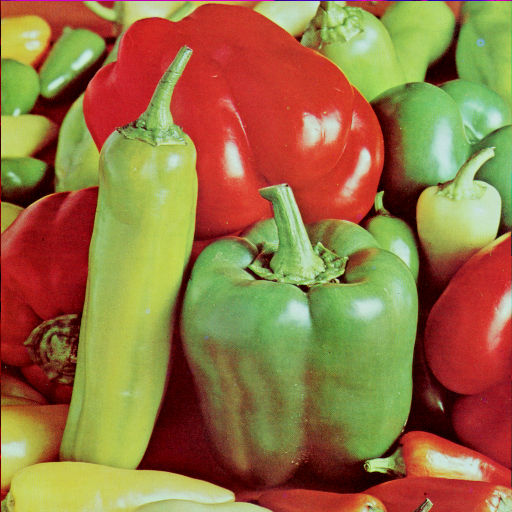
\includegraphics[width=0.45\textwidth]{media/pepper.png}}
  \hspace{0.05\textwidth}
  \subfloat[$\mathcal{I}_{2}$]{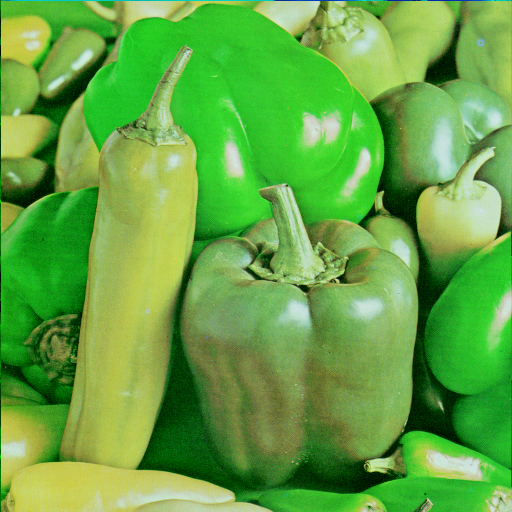
\includegraphics[width=0.45\textwidth]{media/pepper2.png}}
  \caption{Images to be blended.}
\end{figure}
The most obvious method to transition from one image to another is just do exactly that\textemdash just stop showing one image and show the other. But this is a very discrete transition, furthermore, it isn't very friendly on the eye. In spaghetti speak: we ah want to see ah the transition! Hence, we must find a way to slowly change from one image to another, such that if the transition were to take long enough, you would not even notice the change unless you looked at a start and finish frame\textemdash yes, we are indeed looking for \textit{that} level of continuity and smoothness.
\subsection{The Mechanism} Recall a problem of a similar (yet four dimensional) vein: massless particle integration over a discrete wind vector field for HAB path prediction.\\
\par\noindent But how is this even remotely a similar problem?!\\
\par\noindent In the Ballet path prediction algorithms, the massless particle (HAB) exists in a \textit{very} ($>15$ km)coarse vector field. Deep inside the bowels of the Ballet library is a spatiotemporal interpolation engine, which takes the concept of interpolation into four dimensions! It is the single dimension version of this that is applicable to our problem. Take some ``in between'' point, $\alpha$, perhaps $0.45$ ($45$\% along the ``line''), between two values, $v_{1,2}$, $27$ and $33$, respectively. To determine what the value of $\alpha$ should be based on its position relative to $v_{1,2}$ and their values, the following equation can be used:
\begin{equation}\label{eq:subtraction-interpolation}
  v_{\alpha} = v_{1} + \alpha\left(v_{2} - v_{1}\right)
\end{equation}
Alternatively, we could use the mathematical equivalent which uses only addition on $v_{1,2}$:
\begin{equation}\label{eq:addition-interpolation}
  v_{\alpha} = v_{1}(1-\alpha)+\alpha v_{2}
\end{equation}
With either equation, we achieve the following result:
\begin{multline}
  v_{\alpha}=\\
  27 + 0.45\left(33-27\right)\\
  27+2.7\\
  =29.7
\end{multline}
\begin{multline}
  v_{\alpha}=\\
  27\left(1-0.45\right)+0.45\cdot 33\\
  14.85+14.85\\
  =29.7
\end{multline}
It should not be too great a leap of logic to subsitute our images $\mathcal{I}_{1,2}$ into either \ref{eq:subtraction-interpolation} or \ref{eq:addition-interpolation}, and utilize scalar multiplication on matrices to accomplish what the equations do:
\begin{equation}
  \mathcal{I}_{\alpha}=\left(1-\alpha\right)\mathcal{I}_{1}+\alpha\mathcal{I}_{2}
\end{equation}
Programmatically, when this is implemented in OpenCV~\cite{opencv_library}
\section{Randomized Vector Fields}
\subsection{\textit{Basic} Art}
Randomized vector fields provide what is (arguably) the simplest introduction to algorithmic art. Even without the intent of being artistic, it is exceptionally easy for elegant and beautiful patterns to arise naturally from everyday applications of vector fields. For instance, the original motivation for this foray into algorithmic art was high altitude balloon (HAB) path predictions\textemdash a classical application of vector fields, though with slight modification. In path prediction, due to the lack of vertical component (in a $i,j,k=N,E,U$ system) in the forecasts provided by major weather services, the only vertical speed which a HAB carries is its ascent rate. This ascent rate is considered constant in thermodynamically naive simulations, and variable in more detailed simulations, though ascent rate change throughout a flight is negligible even with a thermodynamic model. Hence, these simulations provide somewhat of a fitting analogy dynamic algorithmic art, as the vectors in both fields are $\in \mathbb{R}^{2}$.
\begin{figure}[H]
  \centering
  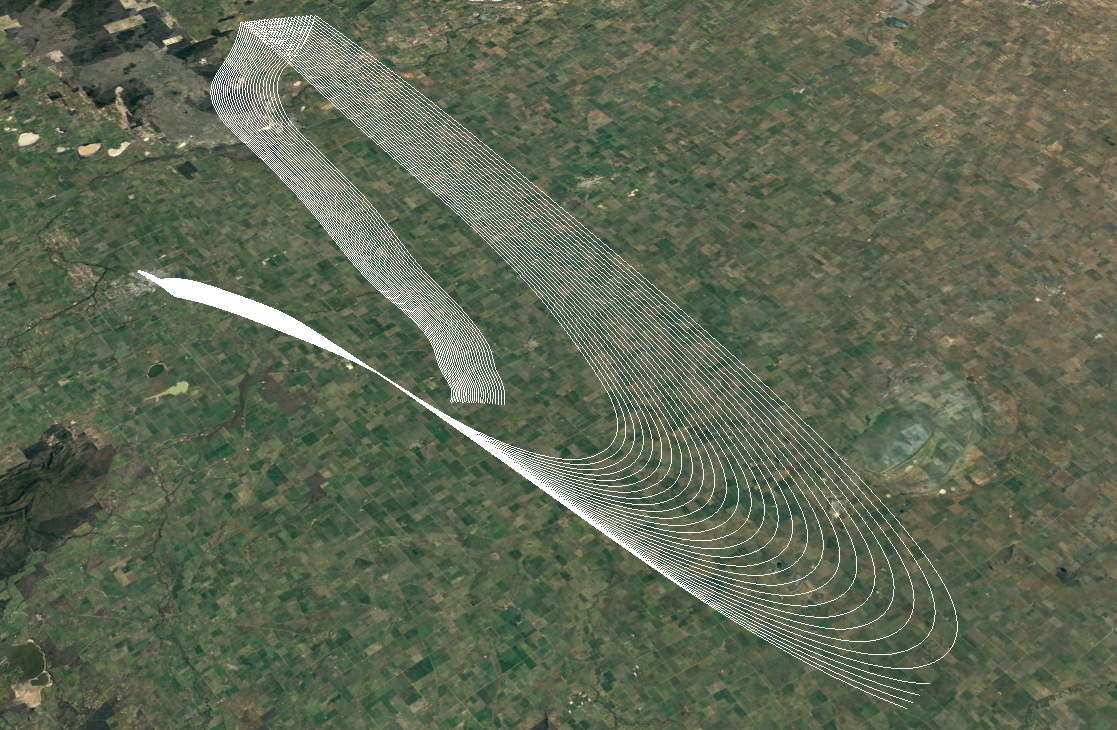
\includegraphics[width=0.9\textwidth]{media/ballet_example.png}
  \caption{A number of predicted paths with varying ascent rate.}
\end{figure}
In the back end of path prediction simulations, the nodes of $\mathbb{R}^{2}$ vectors are $\in \mathbb{R}^{4}$. This allows the experienced wind field to change with time. This is a similar goal for dynamic algorithmic art; multiple frames approaching a representation of a continuously changin, time-variant set of paths. However, in the desired algorithmic art, time brings the field to three dimensions, as frame is two dimensional.
\subsection{Field Generation}
Developing the vector field required for this simple algorithmic art is rather trivial. As mentioned earlier, the field will be three dimensional, with each node being a vector $\in \mathbb{R}^{2}$. Developing this field begins with establishing an order for the dimensions of the field. For the sake of programmatic ease, the field is ordered $t,i,j$. With this structure, insertion of $\mathbb{R}^{2}$ vectors into columns, and columns into fields, and fields into time stacks can be done with nested stacks of C++ \texttt{std::vector} elements, like so:

\begin{algorithm}[H]
  $cells \in \mathbb{Z}^{2}_{+}$\\
  $grid = cells + \left[1,1\right]$\\
  $t_{steps} \in \mathbb{Z}_{+}$\\
  $T$
  \For{$t = 0; t \leq t_{steps}$}
  {
    \For{$i = 0; i \leq cells_{1}$}
    {
      \For{$j = 0; j \leq cells_{2}$}
      {
        test
      }
    }
  }

\caption{Example code}
\end{algorithm}

\bibliography{ref}
\bibliographystyle{IEEEtran}

\end{document}
